\chapter{4位加法器}

\section{第一步：解决什么问题}

加法是所有算术运算的基础。

\begin{itemize}
  \item 减法 = 加法（补码）
  \item 乘法 = 重复加法
  \item 除法 = 重复减法 = 重复加法
  \item ALU的核心 = 加法器
\end{itemize}

\begin{keypoint}[加法器的本质]
加法器 = 实现两个二进制数的加法

$$A + B + C_{in} = Sum + C_{out}$$

每一位：三个输入（$A_i, B_i, C_{in}$）、两个输出（$Sum_i, C_{out}$）
\end{keypoint}

\section{第二步：输入输出关系}

4位加法器：

\begin{itemize}
  \item \textbf{数据输入}：$A_3A_2A_1A_0$（4位），$B_3B_2B_1B_0$（4位），$C_{in}$
  \item \textbf{数据输出}：$S_3S_2S_1S_0$（4位和），$C_{out}$（进位输出）
  \item \textbf{功能}：$A + B + C_{in} = C_{out}S_3S_2S_1S_0$（5位结果）
\end{itemize}

\section{第三步：一位全加器——最基本的加法单元}

在讨论4位加法器之前，必须先理解\textbf{1位全加器（Full Adder, FA）}。

\textbf{1位全加器真值表}：

\begin{center}
\begin{tabular}{|c|c|c||c|c|}
\hline
$A_i$ & $B_i$ & $C_{in}$ & $S_i$ & $C_{out}$ \\
\hline
0 & 0 & 0 & 0 & 0 \\
0 & 0 & 1 & 1 & 0 \\
0 & 1 & 0 & 1 & 0 \\
0 & 1 & 1 & 0 & 1 \\
1 & 0 & 0 & 1 & 0 \\
1 & 0 & 1 & 0 & 1 \\
1 & 1 & 0 & 0 & 1 \\
1 & 1 & 1 & 1 & 1 \\
\hline
\end{tabular}
\end{center}

逻辑表达式：

\begin{align}
  S_i &= A_i \oplus B_i \oplus C_{in} \quad \text{（三输入异或）}\\
  C_{out} &= A_i B_i + A_i C_{in} + B_i C_{in} \quad \text{（三中取二的多数表决）}
\end{align}

\section{第四步：行波进位加法器（Ripple Carry Adder）}

将4个1位全加器串联起来：

\begin{center}
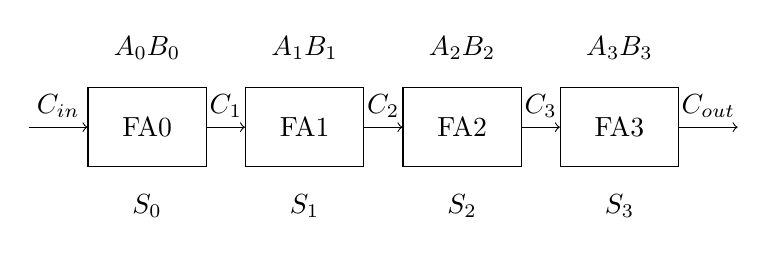
\begin{tikzpicture}
  \node[draw, minimum width=1.5cm, minimum height=1cm] (fa0) at (0,0) {FA0};
  \node[draw, minimum width=1.5cm, minimum height=1cm] (fa1) at (2,0) {FA1};
  \node[draw, minimum width=1.5cm, minimum height=1cm] (fa2) at (4,0) {FA2};
  \node[draw, minimum width=1.5cm, minimum height=1cm] (fa3) at (6,0) {FA3};

  % Carry chain
  \draw[->] (fa0.east) -- node[above] {$C_1$} (fa1.west);
  \draw[->] (fa1.east) -- node[above] {$C_2$} (fa2.west);
  \draw[->] (fa2.east) -- node[above] {$C_3$} (fa3.west);
  \draw[->] (-1.5,0) -- node[above] {$C_{in}$} (fa0.west);
  \draw[->] (fa3.east) -- node[above] {$C_{out}$} (7.5,0);

  % Inputs
  \node at (0,1) {$A_0 B_0$};
  \node at (2,1) {$A_1 B_1$};
  \node at (4,1) {$A_2 B_2$};
  \node at (6,1) {$A_3 B_3$};

  % Outputs
  \node at (0,-1) {$S_0$};
  \node at (2,-1) {$S_1$};
  \node at (4,-1) {$S_2$};
  \node at (6,-1) {$S_3$};
\end{tikzpicture}
\end{center}

\textbf{关键特点}：每个FA的$C_{out}$接到下一个FA的$C_{in}$。进位像水波一样从低位向高位逐级传递。

\textbf{因此得名：Ripple Carry（行波进位/脉动进位）。}

\section{第五步：结构化设计}

4位行波进位加法器 = 4个FA + 进位链：

\begin{itemize}
  \item 每位独立计算本位的 $S_i$ 和 $C_{i+1}$
  \item 进位 $C_i$ 从低位传到高位
  \item 最关键的路径 = 进位链路径（从 $C_{in}$ 到 $C_{out}$ 经过4个FA）
\end{itemize}

\textbf{延迟分析}：
\begin{itemize}
  \item 每个FA的进位延迟 = 2个门延迟（1个AND + 1个OR）
  \item 4位加法器进位延迟 = $4 \times 2 = 8$个门延迟
  \item $S_3$需要等$C_3$稳定后才能计算
\end{itemize}

\section{第六步：为什么这样设计}

\begin{enumerate}
  \item \textbf{为什么进位要逐位传递？}

  因为低位的结果（是否有进位）直接影响高位的计算。这是二进制的内在性质：加法有进位传播。

  \item \textbf{行波进位的优缺点？}

  \textbf{优点}：结构简单、面积小
  \textbf{缺点}：速度慢（进位链延迟随位宽线性增长）

  \item \textbf{为什么还有超前进位加法器（Carry Lookahead）？}

  为突破行波进位速度限制而设计——提前并行计算所有进位，不等待进位传递。但考试通常只考行波进位。
\end{enumerate}

\section{第七步：考试常见变式}

\begin{enumerate}
  \item \textbf{变式1：8位/16位加法器（级联4位加法器）}

  低位加法器的 $C_{out}$ 接到高位加法器的 $C_{in}$。

  \item \textbf{变式2：减法器（用加法器实现减法）}

  $A - B = A + (\sim B + 1)$ = $A + \text{补码}(B)$

  将B取反，$C_{in}=1$，则：$A + (\sim B) + 1 = A - B$。

  \item \textbf{变式3：加法器 + 寄存器 = 累加器}

  每个时钟周期：$ACC \leftarrow ACC + Input$——计数器的基础！

  \item \textbf{变式4：带溢出检测的加法器}

  溢出条件（有符号数）：两个正数相加得负数，或两个负数相加得正数。

  $Overflow = (A_3 \odot B_3) \cdot (A_3 \oplus S_3)$（最高位的符号变化）

  \item \textbf{变式5：BCD加法器}

  二进制加法后如果结果>9，则+6修正。$C_{out} = (S > 9)$ 或 $(C_{out\_binary} = 1)$。
\end{enumerate}

\section{第八步：VHDL实现}

\begin{lstlisting}[caption={4位加法器VHDL实现（行为级）}]
library ieee;
use ieee.std_logic_1164.all;
use ieee.std_logic_unsigned.all;  -- 需要此包以支持算术运算

entity adder_4bit is
  port (
    A    : in  std_logic_vector(3 downto 0);
    B    : in  std_logic_vector(3 downto 0);
    Cin  : in  std_logic;
    Sum  : out std_logic_vector(3 downto 0);
    Cout : out std_logic
  );
end adder_4bit;

architecture behavioral of adder_4bit is
  signal result : std_logic_vector(4 downto 0);
begin
  result <= ('0' & A) + ('0' & B) + Cin;
  Sum  <= result(3 downto 0);
  Cout <= result(4);
end behavioral;
\end{lstlisting}

\begin{lstlisting}[caption={结构级实现（4个全加器级联）}]
architecture structural of adder_4bit is
  signal carry : std_logic_vector(4 downto 0);

  component full_adder is
    port (A, B, Cin : in std_logic; Sum, Cout : out std_logic);
  end component;
begin
  carry(0) <= Cin;

  gen_fa: for i in 0 to 3 generate
    fa_i: full_adder port map (
      A    => A(i),
      B    => B(i),
      Cin  => carry(i),
      Sum  => Sum(i),
      Cout => carry(i+1)
    );
  end generate;

  Cout <= carry(4);
end structural;
\end{lstlisting}

\section{第九步：Testbench验证}

\begin{lstlisting}[caption={4位加法器Testbench}]
library ieee;
use ieee.std_logic_1164.all;
use ieee.std_logic_unsigned.all;

entity adder_4bit_tb is
end adder_4bit_tb;

architecture test of adder_4bit_tb is
  signal A, B, Sum : std_logic_vector(3 downto 0);
  signal Cin, Cout : std_logic;

  component adder_4bit is
    port (
      A    : in  std_logic_vector(3 downto 0);
      B    : in  std_logic_vector(3 downto 0);
      Cin  : in  std_logic;
      Sum  : out std_logic_vector(3 downto 0);
      Cout : out std_logic
    );
  end component;
begin
  uut: adder_4bit port map (A, B, Cin, Sum, Cout);

  stimulus: process
  begin
    Cin <= '0';
    A <= "0011"; B <= "0101"; wait for 10 ns;  -- 3+5=8
    A <= "1010"; B <= "0110"; wait for 10 ns;  -- 10+6=16 -> Cout=1
    A <= "1111"; B <= "0001"; wait for 10 ns;  -- 15+1=16 -> Cout=1
    A <= "0000"; B <= "0000"; wait for 10 ns;  -- 0+0=0
    wait;
  end process;
end test;
\end{lstlisting}

\section{第十步：如何快速解题}

\begin{examtip}[加法器快速解题法]
\begin{enumerate}
  \item \textbf{行为级VHDL}：直接用 \texttt{+} 运算符，最简洁
  \item \textbf{结构级}：generate循环实例化FA，进位链串联
  \item \textbf{减法}：$\sim B + 1 + A$ = $A - B$
  \item \textbf{常考组合}：加法器 + 寄存器 = 累加器（计数器的基础！）
  \item \textbf{溢出判断}：有符号数用$C_{n} \oplus C_{n-1}$，无符号数用$C_{out}$
\end{enumerate}
\end{examtip}

\section{变式详解}
\chapter{4位加法器——5大变式详解}

\section{变式1：8位/16位加法器（级联）}

\begin{detailbox}[完整教学]
\textbf{【方案】}两片4位加法器级联。低位$C_{out}$→高位$C_{in}$。

\textbf{【VHDL——结构级】}
\begin{lstlisting}
add_lo: entity work.adder_4bit port map(A=>A(3 downto 0), B=>B(3 downto 0),
        Cin=>'0', Sum=>Sum(3 downto 0), Cout=>carry);
add_hi: entity work.adder_4bit port map(A=>A(7 downto 4), B=>B(7 downto 4),
        Cin=>carry, Sum=>Sum(7 downto 4), Cout=>Cout);
\end{lstlisting}

\textbf{【行为级——推荐】}
\begin{lstlisting}
signal result : std_logic_vector(8 downto 0);
result <= ('0' & A) + ('0' & B);
Sum <= result(7 downto 0); Cout <= result(8);
\end{lstlisting}
综合器自动优化任意位宽加法。
\end{detailbox}


\section{变式2：减法器（用加法器实现A-B）}

\begin{detailbox}[完整教学]
\textbf{【补码原理】}$A-B = A+(-B) = A+(\sim B+1) = A+\sim B+1$

\textbf{【电路】}B取反→接加法器B输入。$C_{in}=1$（实现+1）。$C_{in}$就是补码中的"+1"。

\textbf{【VHDL】}
\begin{lstlisting}
diff <= A + (not B) + '1';  -- A-B = A + (~B) + 1
-- 或直接用减法运算符
diff <= A - B;
\end{lstlisting}

\begin{examfocus}
\textbf{常考}：为什么$C_{in}=1$能实现减法？
答案：$A-B = A+(\sim B)+1$ → +1部分由$C_{in}=1$提供。
\end{examfocus}
\end{detailbox}


\section{变式3：加法器+寄存器=累加器}

\begin{detailbox}[完整教学]
\textbf{【结构】}加法器计算$ACC+Input$。结果在时钟沿存入ACC。ACC输出反馈回加法器输入端。

\textbf{【VHDL】}
\begin{lstlisting}
process(clk, rst_n)
begin
  if rst_n='0' then acc <= (others=>'0');
  elsif rising_edge(clk) then
    acc <= acc + input_data;  -- 每个时钟累加一次
  end if;
end process;
\end{lstlisting}

\textbf{【本质】}累加器=计数器的一种（不是每次+1，而是+任意值）。

\textbf{【应用】}DSP中的乘累加(MAC)、积分器。
\end{detailbox}


\section{变式4：带溢出检测的加法器}

\begin{detailbox}[完整教学]
\textbf{【无符号数溢出】}$C_{out}=1$=溢出（结果超过最大值）。

\textbf{【有符号数溢出】}$Overflow = C_n \oplus C_{n-1}$（最高位进位和次高位进位异或）。

\textbf{【VHDL】}
\begin{lstlisting}
signal result : std_logic_vector(4 downto 0);  -- 5位
result <= ('0' & A) + ('0' & B);
Sum <= result(3 downto 0);
Cout <= result(4);
-- 有符号溢出
Overflow <= result(4) xor result(3);  -- C4 xor C3
\end{lstlisting}

\textbf{【直观判断】}
两个正数相加得负数 → 溢出 (正溢出)
两个负数相加得正数 → 溢出 (负溢出)
\end{detailbox}


\section{变式5：BCD加法器}

\begin{detailbox}[完整教学]
\textbf{【问题】}二进制加法后，如果结果>9(1001)，需要+6(0110)修正为BCD格式。

\textbf{【VHDL】}
\begin{lstlisting}
signal bin_sum : std_logic_vector(4 downto 0);
signal bcd_sum : std_logic_vector(3 downto 0);
begin
  bin_sum <= ('0' & A) + ('0' & B);
  bcd_sum <= bin_sum(3 downto 0) when bin_sum <= 9
        else bin_sum(3 downto 0) + "0110";  -- >9时+6修正
  Cout <= '1' when bin_sum > 9 else '0';
\end{lstlisting}

\textbf{【例子】}5+7=12(1100)。1100+0110=10010→BCD: 0001 0010(12)。
\end{detailbox}
